\documentclass[a4paper]{article}
\usepackage{amsmath}
\usepackage{graphicx}
\usepackage{geometry}
\usepackage{floatrow}
\usepackage{layout}
\usepackage{amssymb} 
\usepackage{multirow}
\usepackage{caption}
\geometry{margin=1in}
\usepackage{authblk}
\usepackage{indentfirst}
\usepackage[hidelinks]{hyperref}
\usepackage{enumitem}
\usepackage{float}
\usepackage{hyperref}
\usepackage{amssymb}
\usepackage{xcolor}
\usepackage{titlesec}
\usepackage{tikz} 


% Define link color
\hypersetup{
    colorlinks=true,
    linkcolor=teal,  % Color for internal links
    filecolor=teal,  % Color for file links
    urlcolor=teal,   % Color for URLs
    citecolor=black  % Color for citation links
}

% Define custom dark teal color
\definecolor{darkteal}{RGB}{0, 102, 102}

% Define section color
\titleformat{\section}
  {\color{darkteal}\normalfont\Large\bfseries} % Formatting for section titles
  {\thesection}{1em}{}

\providecommand{\keywords}[1]
{
  \small	
  \textbf{\; \textit{Keywords---}} #1
}

\begin{document}

\title{\textbf{\huge{Problem Set 2}}}

\author{\textbf\large{Teera Tesharojanasup}}

\affil{\textbf{Northeastern University, Boston}}

\date{\text{July 23rd, 2024}}

\maketitle
\begin{sloppypar}

\section*{Overview}

Problem set 2 for CS 4100 Summer II. Taught by assistant teaching professor, \href{https://rajagopalvenkat.com/}{Rajagopal Venkat}. \cite{MISC:1}

\section{Markov Models}

\par Consider the following Markov model with 3 states, \textbf{S1}, \textbf{S2} and \textbf{S3}. The transition probabilities of the model are 
represented along the edges (note that each edge is directional).

\begin{figure}[H]
    \centering  
    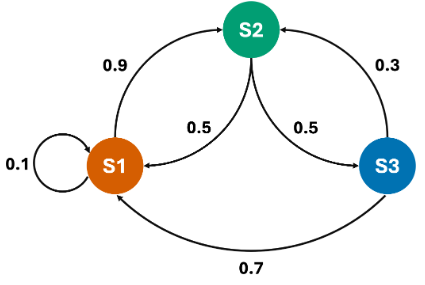
\includegraphics[height=0.2\textheight]{markov_model.png}
    \label{fig:markov_model}
\end{figure}

\begin{enumerate}[start=1,label=Q\arabic*,left=0pt]
    \item \textbf{Given the above Markov model, explain whether the stationary distribution depends on the start state (without actually computing the stationary distribution). \hfill \textcolor{teal}{(2)}}
    
    \par Given the above Markov model, the stationary distribution does not depend on the start state. Given any start state,
    the probability distribution will converge towards the stationary distribution as $n$ grows larger as long as there is a path that
    exists between any two states which the Markov model above satisfies.
    
    \item \textbf{Given the initial probability distribution} $p_0 = [0.1, 0.6, 0.3]$ \textbf{for states} $S1, S2,$ \textbf{and} $S3$ \textbf{respectively, compute the stationary distribution for the given Markov model. You may use a program to do the computations. Report only the final stationary distribution ${\pi}$. \hfill \textcolor{teal}{(2)}}

    \par $ \pi = [0.38636364, \: 0.40909091, \: 0.20454545] $
    
    \item \textbf{What is the probability of the following transition sequence: $S1 \rightarrow S1 \rightarrow S2 \rightarrow S3?$ (Use the stationary distribution computed above, and show your calculations.) \hfill \textcolor{teal}{(2)}}
    \begin{align*}
        & \hfill \text{Probability of starting at S1} \hfill = 0.3864 \\\\
        P(S1 \rightarrow S1 \rightarrow S2 \rightarrow S3) &= \text{(Probability of starting at S1)} \cdot P(S1 | S1) \cdot P(S2 | S1) \cdot P(S3 | S2) \\
        P(S1 \rightarrow S1 \rightarrow S2 \rightarrow S3) &= 0.3864 \cdot 0.1 \cdot 0.9 \cdot 0.5 \\
        P(S1 \rightarrow S1 \rightarrow S2 \rightarrow S3) &= 0.017388
    \end{align*}
    
    \item \textbf{Given that we start in the state $S2$, what is the probability of returning to $S2$ after two transitions? (Show your calculations.) \hfill \textcolor{teal}{(2)}}
    \begin{align*}
        & \hfill \text{Probability of starting at S2} \hfill = 0.409 \\\\
        P(S2 \rightarrow X \rightarrow S2) &= P(S2 \rightarrow S1 \rightarrow S2) + P(S2 \rightarrow S2 \rightarrow S2) + P(S2 \rightarrow S3 \rightarrow S2) \\
        P(S2 \rightarrow X \rightarrow S2) &= (0.409 \cdot 0.5 \cdot 0.9) + (0.409 \cdot 0 \cdot 0) + (0.409 \cdot 0.5 \cdot 0.3) \\
        P(S2 \rightarrow X \rightarrow S2) &= 0.2454
    \end{align*}

    \item \textbf{Given the starting probability distribution $p_0 = [0.1, 0.6, 0.3]$, what is the probability of ending up in $S2$ after exactly two transitions? (Show your calculations.) \hfill \textcolor{teal}{(2)}}
    \begin{align*}
        & \hfill \text{Probability of starting at S1} \hfill = 0.1 \\
        & \hfill \text{Probability of starting at S2} \hfill = 0.6 \\
        & \hfill \text{Probability of starting at S3} \hfill = 0.3 \\\\
        P(X \rightarrow Y \rightarrow S2) &= P(S1 \rightarrow S1 \rightarrow S2) + P(S1 \rightarrow S2 \rightarrow S2) + P(S1 \rightarrow S3 \rightarrow S2) \\
        &\quad + P(S2 \rightarrow S1 \rightarrow S2) + P(S2 \rightarrow S2 \rightarrow S2) + P(S2 \rightarrow S3 \rightarrow S2) \\
        &\quad + P(S3 \rightarrow S1 \rightarrow S2) + P(S3 \rightarrow S2 \rightarrow S2) + P(S3 \rightarrow S3 \rightarrow S2) \\\\
        &= (0.1 \cdot 0.1 \cdot 0.9) + (0.1 \cdot  0.9 \cdot 0) + (0.1 \cdot 0 \cdot 0.3) \\
        &\quad + (0.6 \cdot 0.5 \cdot 0.9) + (0.6 \cdot 0 \cdot  0) + (0.6 \cdot 0.5 \cdot 0.3) \\
        &\quad + (0.3 \cdot 0.7 \cdot 0.9) + (0.3 \cdot 0.3 \cdot 0) + (0.3 \cdot 0 \cdot 0.3) \\\\
        &= 0.558
    \end{align*}

\end{enumerate}

\section{Hidden Markov Models}

Recall Hidden Markov Models (HMM) from class, where we applied this approach to sequence 
labeling tasks such as parts-of-speech tagging or named entity recognition. Here,
your task is to construct and use an HMM model to make inferences about a coin-flipping
game with the following rules. \\

\noindent Your professor produces two identical looking coins. However, only one of the coins is a
fair coin, and the other is a biased coin that produces an outcome of \textbf{Heads} 70\% of the
time. The professor always knows which coin is the fair one, and will perform three coin
flips in total. Between each flip, the professor may swap the coin, following the rule that
if a fair coin is flipped in one round, then in the next round, the professor chooses a coin
completely at random. If, however, the biased coin is flipped in any round, then the professor 
is twice as likely to choose the biased coin again in the next round, as compared to
the fair coin. As the three flips are performed, you observe the outcomes \textbf{Heads}, \textbf{Heads}
and \textbf{Tails} respectively.


\begin{enumerate}[start=6,label=Q\arabic*,left=0pt]
    \item \textbf{Draw the HMM diagram for this game showing transitions between hidden states,
    and emissions to outcomes with the corresponding probabilities labeled along the edges.
    Hand-drawn figures accepted for this question, provided the grader can read everything
    clearly. (For reference, see \href{https://rajagopalvenkat.com/teaching/resources/AI/ch6.html\#hmm}{the second diagram in our HMM notes}, showing the Very Late,
    Late and On Time hidden states, and the Happy and Sad outcomes.) \hfill \textcolor{teal}{(5)}}

    \begin{figure}[H]
        \centering  
        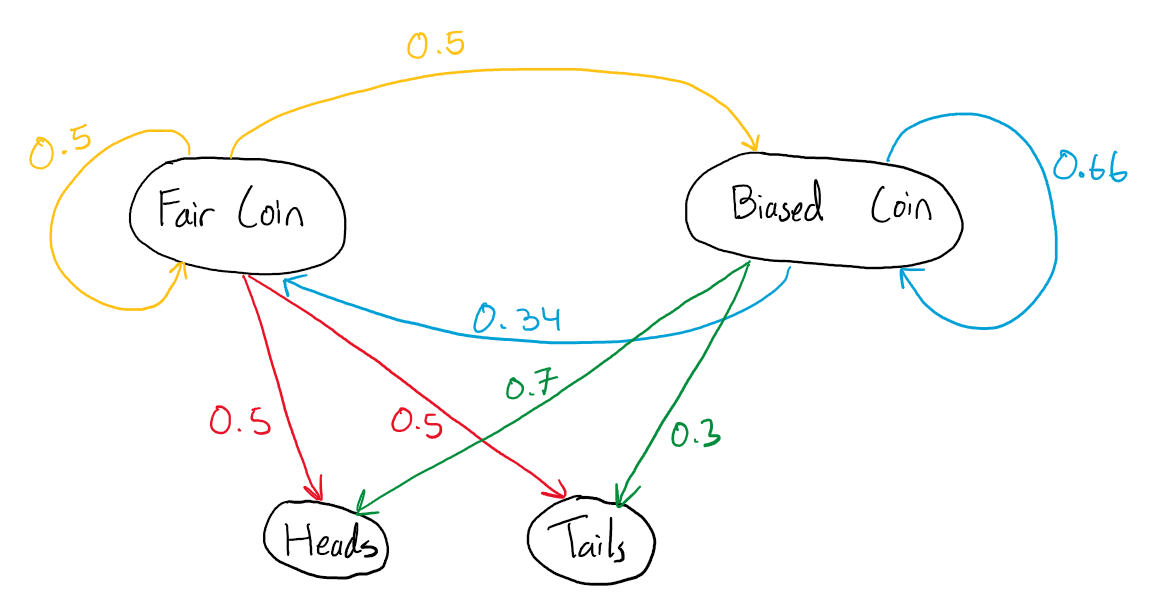
\includegraphics[height=0.3\textheight]{Q6_hmm.png}
        \label{fig:Q6_hmm}
    \end{figure}

    \item \textbf{Given the observed outcome sequence, predict which coin was most likely flipped
    in each of the three turns (i.e., compute the most likely hidden sequence). Show all your
    intermediate calculations and use the stationary distribution to reason about which coin
    was flipped in the very first round. \hfill \textcolor{teal}{(10)}}

    \begin{center}
        \fbox{FC = Fair Coin, BC = Biased Coin, H = Heads, T = Tails}
        \fbox{%
        \begin{minipage}{0.7\textwidth}
            \[
                Transition \: Matrix = 
                \bordermatrix{ & FC & BC \cr
                FC & 0.5 & 0.5 \cr
                BC & 0.34 & 0.66 }
            \]
    
            \[
                Observation \: Matrix = 
                \bordermatrix{ & H & T \cr
                H & 0.5 & 0.5 \cr
                T & 0.7 & 0.3 }
            \]
    
            \[ 
                Stationary \: Distribution: \pi = [0.4047619, \: 0.5952381] 
            \]
        \end{minipage}%
        }
    \end{center}

    \begin{align*}
        & \textbf{One Sequence Permutations}: \\\\
        %%% 1st
        & FC \\
        & \downarrow \quad P(Start \: FC) \cdot P(H | FC) = 0.4048 \cdot 0.5 = 0.2024 \\
        & H \\\\
        %%% 2nd
        & BC \\
        & \downarrow \quad P(Start \: BC) \cdot P(H | BC) = 0.5952 \cdot 0.7 = 0.4166 \\
        & H \\\\
    \end{align*}

    \begin{align*}
        & \textbf{Two Sequence Permutations}: \\\\
        %%% 1st
        & FC \rightarrow FC \\
        & \downarrow \quad \quad \quad \downarrow \quad 0.2024 \cdot P(FC | FC) \cdot P(H | FC) = 0.2024 \cdot 0.5 \cdot 0.5 = 0.0506 \\
        & H \quad \quad \:\:\: H \\\\
        %%% 2nd
        & BC \rightarrow FC \\
        & \downarrow \quad \quad \quad \downarrow \quad 0.4166 \cdot P(FC | BC) \cdot P(H | FC) = 0.4166 \cdot 0.34 \cdot 0.5 = 0.0708 \\
        & H \quad \quad \:\:\: H \\\\
        %%% 3rd
        & FC \rightarrow BC  \\
        & \downarrow \quad \quad \quad \downarrow \quad 0.2024 \cdot P(BC | FC) \cdot P(H | BC) = 0.2024 \cdot 0.5 \cdot 0.7 = 0.0708 \\
        & H \quad \quad \:\:\: H \\\\
        %%% 4th
        & BC \rightarrow BC \\
        & \downarrow \quad \quad \quad \downarrow \quad 0.4166 \cdot P(BC | BC) \cdot P(H | BC) = 0.4166 \cdot 0.66 \cdot 0.7 = 0.1925 \\
        & H \quad \quad \:\:\: H
    \end{align*}

    \begin{align*}
        & \textbf{Three Sequence Permutations}: \\\\
        %%% 1st
        & FC \rightarrow FC \rightarrow FC \\
        & \downarrow \quad \quad \quad \downarrow \quad \quad \quad \downarrow \quad 0.0506 \cdot P(FC | FC) \cdot P(T | FC) = 0.0506 \cdot 0.5 \cdot 0.5 = 0.01265 \\
        & H \quad \quad \:\:\: H \quad \quad \:\:\: T \\\\
        %%% 2nd
        & FC \rightarrow FC \rightarrow BC \\
        & \downarrow \quad \quad \quad \downarrow \quad \quad \quad \downarrow \quad 0.0506 \cdot P(BC | FC) \cdot P(T | BC) = 0.0506 \cdot 0.5 \cdot 0.3 = 0.0076 \\
        & H \quad \quad \:\:\: H \quad \quad \:\:\: T \\\\
        %%% 3rd
        & FC \rightarrow BC \rightarrow FC \\
        & \downarrow \quad \quad \quad \downarrow \quad \quad \quad \downarrow \quad 0.0708 \cdot P(FC | BC) \cdot P(T | FC) = 0.0708 \cdot 0.34 \cdot 0.5 = 0.0120 \\
        & H \quad \quad \:\:\: H \quad \quad \:\:\:T \\\\
        %%% 4th
        & FC \rightarrow BC \rightarrow BC \\
        & \downarrow \quad \quad \quad \downarrow \quad \quad \quad \downarrow \quad 0.0708 \cdot P(BC | BC) \cdot P(T | BC) = 0.0708 \cdot 0.66 \cdot 0.3 = 0.0140 \\
        & H \quad \quad \:\:\: H \quad \quad \:\:\: T \\\\
        %%% 5th
        & BC \rightarrow FC \rightarrow FC \\
        & \downarrow \quad \quad \quad \downarrow \quad \quad \quad \downarrow \quad 0.0708 \cdot P(FC | FC) \cdot P(T | FC) = 0.0708 \cdot 0.5 \cdot 0.5 = 0.0177 \\
        & H \quad \quad \:\:\: H \quad \quad \:\:\: T \\\\
        %%% 6th
        & BC \rightarrow FC \rightarrow BC \\
        & \downarrow \quad \quad \quad \downarrow \quad \quad \quad \downarrow \quad 0.0708 \cdot P(BC | FC) \cdot P(T | BC) = 0.0708 \cdot 0.5 \cdot 0.3 = 0.0106 \\
        & H \quad \quad \:\:\: H \quad \quad \:\:\: T \\\\
        %%% 7th
        & BC \rightarrow BC \rightarrow FC \\
        & \downarrow \quad \quad \quad \downarrow \quad \quad \quad \downarrow \quad 0.1925 \cdot P(FC | BC) \cdot P(T | FC) = 0.1925 \cdot 0.34 \cdot 0.5 = 0.0327 \\
        & H \quad \quad \:\:\: H \quad \quad \:\:\: T \\\\
        %%% 8th
        & BC \rightarrow BC \rightarrow BC \\
        & \downarrow \quad \quad \quad \downarrow \quad \quad \quad \downarrow \quad 0.1925 \cdot P(BC | BC) \cdot P(T | BC) = 0.1925 \cdot 0.66 \cdot 0.3 = 0.0381 \\
        & H \quad \quad \:\:\: H \quad \quad \:\:\: T
    \end{align*}

    \par According to $\pi$, it is more likely that the biased coin was flipped in the initial round. \newline   

    $\therefore$ The most likely sequence of coin types that were flipped to get H, H, T were BC, BC, BC 
    with a probability of 0.0381.

\end{enumerate}

\section{Markov Decision Processes and Reinforcement Learning}

Consider the following MDP with 4 states, and 4 actions. A dashed line represents a
transition from a chosen action to some next state. Transition probabilities are specified
along each dashed edge.

\begin{figure}[H]
    \centering  
    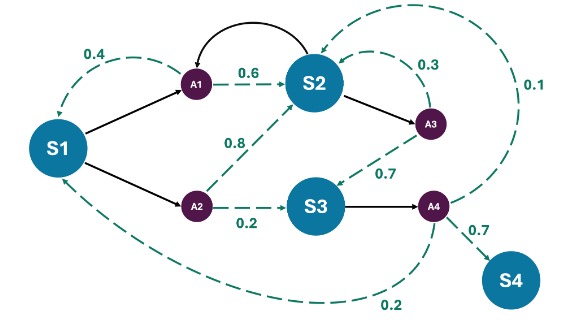
\includegraphics[height=0.3\textheight]{mdp_and_rl.png}
    \label{fig:mdp_and_rl}
\end{figure}

\begin{enumerate}[start=8,label=Q\arabic*,left=0pt]
    \item \textbf{How many unique policies does this MDP have? Explain your reasoning and list all policies. Use $X$ to indicate no possible action from a state. \hfill \textcolor{teal}{(2)}}
    
    \begin{table}[h!]
    \centering
    \begin{tabular}{ |c|c|c|c| } 
        \hline
        S1 & S2 & S3 & S4 \\
        \hline
        A1 & A1 & A4 & X \\ 
        A1 & A3 & A4 & X \\ 
        A2 & A1 & A4 & X \\ 
        A2 & A3 & A4 & X \\ 
        \hline
    \end{tabular}
    \caption{Table showing 4 unique policies}
    \label{table:1}
    \end{table}

    We can create a table to see which combination of policies each state can take and we end up
    with 4 unique policies.
    
    \item \textbf{If from any state, all valid actions are equally likely, then what is the total probability
    of reaching S4 from S1 using paths of at most length 3? List all such paths and compute
    the total probability. Show your calculations. (An action followed by a transition into a next
    state counts as a total of one move.) \hfill \textcolor{teal}{(4)}}
    
    \begin{align*}
        \textbf{Path 1}&: S1 \rightarrow (A1 \:\: S2) \rightarrow (A3 \:\: S3) \rightarrow (A4 \:\: S4) \\
        &= P(A1 | S1) \cdot P(S2 | A1) \cdot P(A3 | S2) \cdot P(S3 | A3) \cdot P(A4 | S3) \cdot P(S4 | A4) \\
        &= 0.5 \cdot 0.6 \cdot 0.5 \cdot 0.7 \cdot 1.0 \cdot 0.7 \\
        &= 0.0735 \\\\
        \textbf{Path 2}&: S1 \rightarrow (A2 \:\: S2) \rightarrow (A3 \:\: S3) \rightarrow (A4 \:\: S4) \\
        &= P(A2 | S1) \cdot P(S2 | A2) \cdot P(A3 | S2) \cdot P(S3 | A3) \cdot P(A4 | S3) \cdot P(S4 | A4) \\
        &= 0.5 \cdot 0.8 \cdot 0.5 \cdot 0.7 \cdot 1 \cdot 0.7 \\
        &=  0.098 \\\\
        \textbf{Path 3}&: S1 \rightarrow (A2 \:\: S3) \rightarrow (A4 \:\: S4) \\
        &= P(A2 | S1) \cdot P(S3 | A2) \cdot P(A4 | S3) \cdot P(S4 | A4) \\
        &= 0.5 \cdot 0.2 \cdot 1 \cdot 0.7 \\
        &= 0.07
    \end{align*}

    $\therefore \:$ There is a $0.0735 + 0.098 + 0.07 = 0.2415$ probability that we can reach S4 from S1 using paths of at most length 3.

    \item \textbf{Given that $R(S1, A1, S2) = 10$, $R(S1, A2, S2) = 10$, $R(S1, A2, S3) = 15$, $R(S3, A4, S4) = 100$, 
    and that rewards for all other transitions are $0$, write and expand the optimal value
    function equation for $V_{opt}(S1)$. Assume that the discount factor is $\gamma$, and leave your final
    answer in terms of $V_{opt}(S2)$ and $V_{opt}(S3)$. \hfill \textcolor{teal}{(4)}}
    
    \begin{align*}
        & V_{opt}(S1) = \max_{\substack{a}}\left(\sum_{s'}T(S1, a, s')[R(S1, a, s') + \gamma V_{opt}(s')]\right) \\\\
        & \text{For A1:} \\\\
        & = T(S1, A1, S1)[R(S1, A1, S1) + \gamma V_{opt}(S1)] + T(S1, A1, S2)[R(S1, A1, S2) + \gamma V_{opt}(S2)] \\
        & = 0.4[0 + \gamma V_{opt}(S1)] + 0.6[10 + \gamma V_{opt}(S2)] \\
        & = (\gamma 0.4 V_{opt}(S1)) + (6 + \gamma 0.6 V_{opt}(S2)) \\
        & = 6 + \gamma(0.4 V_{opt}(S1) + 0.6 V_{opt}(S2)) \\\\
        & \text{For A2:} \\\\
        & = T(S1, A2, S2)[R(S1, A2, S2) + \gamma V_{opt}(S2)] + T(S1, A2, S3)[R(S1, A2, S3) + \gamma V_{opt}(S3)] \\
        & = 0.8[10 + \gamma V_{opt}(S2)] + 0.2[15 + \gamma V_{opt}(S3)] \\
        & = (8 + \gamma 0.8 V_{opt}(S2)) + (3 + \gamma 0.2 V_{opt}(S3)) \\
        & = 11 + \gamma(0.8 V_{opt}(S2) + 0.2 V_{opt}(S3)) \\\\
        & \therefore \: V_{opt}(S1) = \max_{\substack{a}} \biggl( 6 + \gamma(0.4 V_{opt}(S1) + 0.6 V_{opt}(S2)), 11 + \gamma(0.8 V_{opt}(S2) + 0.2 V_{opt}(S3)) \biggr)
    \end{align*}

    \item \textbf{Assume that by simulating this MDP using some exploration policy $\pi$, we obtain the
    two following episodes:}

    \begin{figure}[H]
        \centering  
        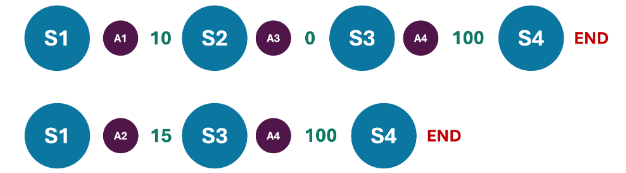
\includegraphics[width=0.8\textwidth]{Q11_mdp.png}
        \label{fig:Q11_mdp}
    \end{figure}

    \textbf{Use Q-learning updates to calculate the agent’s final optimal policy given this data stream,
    and show all intermediate steps. Assume $\gamma = 1$. For your reference, the Q-learning update equation is given by: \hfill \textcolor{teal}{(10)}}
    
    \[ \eta = \frac{1}{1 + \text{number of updates to } \hat{Q}_{opt}(s, a)} \]

    \textbf{For each observed $(s, a, r, s')$:}

    \[ Estimate, \; \hat{Q}^{(t)}_{opt}(s, a) = (1 - \eta) \hat{Q}^{(t-1)}_{opt}(s, a) + \eta[R(s, a, s') + \gamma \hat{V}^{(t-1)}_{opt}(s')] \]
    \[ where \:\: \hat{V}_{opt}(s') = \max_{\substack{a'}} \ \hat{Q}_{opt}(s', a') \]

\end{enumerate}

\section{Academic Integrity}

\begin{enumerate}[start=12,label=Q\arabic*,left=0pt]
    \item \textbf{Review, and copy/paste the following academic integrity acknowledgement in your final submission as the answer to Q12.}
    
    \par I have read and understood the academic integrity policy as outlined in the course syllabus for CS4100. 
    By pasting this acknowledgement in my submission, I declare that all work presented here is my own, and any conceptual 
    discussions I may have had with classmates have been fully disclosed. I declare that generative AI was not used to answer
    any questions in this assignment. Any use of generative AI to improve writing clarity alone is accompanied by an appendix 
    with my original, unedited answers.

\end{enumerate}

\end{sloppypar}

\bibliography{references}
\bibliographystyle{ieeetr}

\end{document}